\section{Random and Mixed Effects Models}

Up to now, treatment effects ($\alpha_i$) where fixed, unknown quantities that we tried to estimate. This means we are making a statement about a specific, fixed set of treatments. Such models are also called \textbf{fixed effects models}.

\subsection{Random Effects Model}

\subsubsection{One-Way ANOVA}

We now consider situations where treatments are random samples from a large population of treatments. \textbf{We are interested in making a statement about some properties of the whole population and not of the observed individuals}. We can model such data with the model
$$Y_{ij} = \mu + \alpha_i + \epsilon_{ij}, \qquad \alpha_i \text{ i.i.d.} \sim \mathcal{N}(0, \sigma_\alpha^2)$$

where $\alpha_i$ is the effect of the $i$ samples, it is also called a \textbf{random effect}. Sometimes, such models are also called \textbf{variance components models}. Let us inspect some properties of the model.

$$\E [Y_{ij}] = \mu \qquad \text{Var}(Y_{ij}) = \sigma_\alpha^2 + \sigma^2$$
$$\text{Cor}(Y_{ij}, Y_{kl}) = \begin{cases}
	0 & i \neq k \\
	\sigma_\alpha^2 / (\sigma_\alpha^2 + \sigma^2) & i = k, j \neq l \\
	1 & i = k, j = l
\end{cases}$$

Observations from different samples are uncorrelated while observations from the same sample are correlated. The correlation within the same sample is also called the intraclass correlation (ICC). When large ($\sigma_\alpha^2 >> \sigma^2$), it means that observations from the same sample are much more similar than observations from different samples.

\begin{center}
	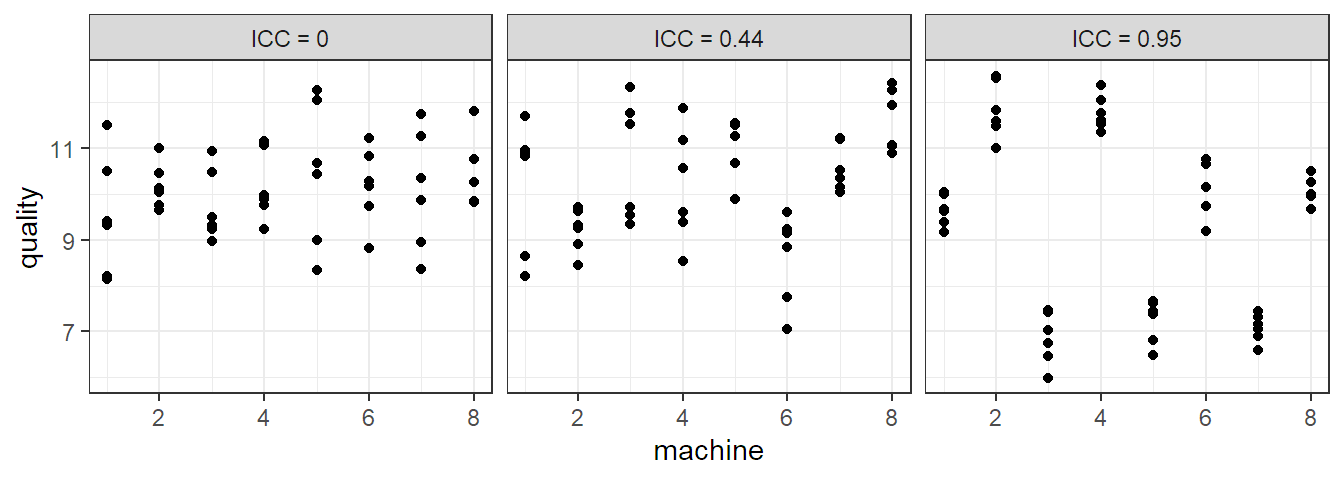
\includegraphics[width=\linewidth]{icc.png}
\end{center}

The same holds for multiple random effects. For them, the correlation is the sum of shared variance components divided by the sum of all variance components. Parameter estimation for the variance components $\sigma_\alpha^2,\, \sigma^2$ is done with the so-called restricted maximum likelihood technique.

\begin{lstlisting}
library(lme4) ## lmerTest would be an alternative
fit <- lmer(y ~ (1 | x), data = d)
## As usual we can use summary and confint
## Linear mixed model fit by REML ['lmerMod']
## ...
## Random effects:
##  Groups   Name         Variance    Std.Dev.
##  x       (Intercept)        117        10.8    
##  Residual                   464        21.5    
## Number of obs: 40, groups:  sire, 5
## 
## Fixed effects:
##             Estimate Std. Error t  value
## (Intercept)    82.55          5.91     14
\end{lstlisting}

Confidence intervals are often larger than with fixed effect models, as we now try to make a statement about a larger population and not only about the measured samples. To verify our model assumptions we can again use QQ-plots:
\begin{lstlisting}
## QQ-plots of random effects
qqnorm(ranef(fit)$x[,1], main = "x")
## QQ-plots of residuals
qqnorm(resid(fit), main = "residuals")
\end{lstlisting}

\subsubsection{More Than One Factor}

So far this was a one-way ANOVA model with a random effect. We can extend this to the two-way ANOVA situation and beyond. For the two-way ANOVA situation we have the following model:
$$Y_{ijk} = \mu + \alpha_i + \beta_j + (\alpha \beta)_{ij} + \epsilon_{ijk}$$

Hereby $\alpha_i$ and $\beta_j$ are the random (main) effects. From here we can apply the same techniques as before.
\begin{lstlisting}
fit <- lmer(y ~ (1 | a) + (1 | b) + (1 | a:b), data = d)
\end{lstlisting}

\subsubsection{Nesting}

We introduce a new data structure, where the level of factor $B$ has a different meaning for every level of factor $A$. The two factors are \textbf{not crossed}, we say $B$ is \textbf{nested} in $A$. We can use the following model:
$$Y_{ijk} = \mu + \alpha_i + \beta_{j(i)} + \epsilon_{ijk}$$

Here $\alpha_i$ is the random effect of $A$ and $\beta_{j(i)}$ is the random effect of $B$ within $A$. We make the usual assumptions for the random effects:
$$\alpha_i \text{ i.i.d.} \sim \mathcal{N}(0, \sigma_\alpha^2), \qquad \beta_{j(i)} \text{ i.i.d.} \sim \mathcal{N}(0, \sigma_\beta^2)$$

\begin{lstlisting}
fit <- lmer(y ~ (1 | a/b), data = d)
## Alternatively
fit <- lmer(y ~ (1 | a) + (1 | a:b), data = d)
\end{lstlisting}

\subsection{Mixed Effects Models}

In practice, we often encounter models which contain both random and fixed effects. We call them \textbf{mixed models} or \textbf{mixed effects models}. Let assume we have a fixed effect $A$ and a random effect $B$. We can model our data as follows:
$$Y_{ijk} = \mu + \alpha_i + \beta_j + (\alpha \beta)_{ij} + \epsilon_{ijk}$$

Here $\alpha_i$ is the fixed effect, $\beta_j$ the random effect and $(\alpha \beta)_{ij}$ the random interaction effect. An interaction effect between a random and a fixed effect is treated as a random effect. We assume that all random effects are normally distributed, this means:
$$\beta_j \text{ i.i.d.} \sim \mathcal{N}(0, \sigma_\beta^2), \qquad (\alpha\beta)_{ji} \text{ i.i.d.} \sim \mathcal{N}(0, \sigma_{\alpha\beta}^2)$$

Now the same techniques can be used again to analyse the fixed effects and the random effects.
\begin{lstlisting}
options(contrasts = c("contr.treatment", "contr.poly"))
library(lmerTest)
fit <- lmer(y ~ a + (1 | b) + (1 | b:a), data = d)
\end{lstlisting}
